\documentclass[presentation]{beamer}
\usepackage[utf8]{inputenc}
\usepackage[T1]{fontenc}
\usepackage{fixltx2e}
\usepackage{graphicx}
\usepackage{longtable}
\usepackage{float}
\usepackage{wrapfig}
\usepackage{rotating}
\usepackage[normalem]{ulem}
\usepackage{amsmath}
\usepackage{textcomp}
\usepackage{marvosym}
\usepackage{wasysym}
\usepackage{amssymb}
\usepackage{hyperref}
\tolerance=1000
\usepackage{graphicx} \DeclareMathOperator{\argmin}{argmin}

\newcommand{\under}[2]{\underset{\scriptscriptstyle#1}{#2}}


\usetheme{simple}
\usecolortheme{}
\usefonttheme{serif}
\useinnertheme{}
\useoutertheme{}
\author{Talon Chandler}
\date{January 17, 2017}
\title{Update On 3D Orientation Reconstruction}

\begin{document}

\maketitle
\begin{frame}[label=sec-1]{Forward model}
\begin{align*}
g_i = \int_{\mathbb{S}^2}d\hat{\textbf{r}}\ h_i(\hat{\textbf{r}})f(\hat{\textbf{r}})
\end{align*}
\begin{itemize}
\item $g_i$ $\rightarrow$ is the $i$th intensity measurement
\item $h_i(\hat{\textbf{r}})$ $\rightarrow$ is the $i$th point response function
\item $f(\hat{\textbf{r}})$ $\rightarrow$ is the orientation distribution function
\end{itemize}
\end{frame}

\begin{frame}{Integral $\rightarrow$ Matrix}
  \begin{align*}
  g_i &= \int_{\mathbb{S}^2}d\hat{\textbf{r}}\ h_i(\hat{\textbf{r}})f(\hat{\textbf{r}})\\ \\
  g_i &= \textbf{H}_i^T\textbf{F}\\ \\
  \mathbf{g} &= \mathbf{\Psi}\textbf{F}
  \end{align*}
\end{frame}

\begin{frame}{Discrete inverse transform matrix $\mathbf{B}$}
  \begin{align*}
    \mathbf{f} = \mathbf{B}\mathbf{F}
  \end{align*}
  where $\mathbf{f}$ is a discrete approximation to the true distribution
  $f(\hat{\textbf{r}})$. $\mathbf{f}$ is an $R\times 1$ vector where $R$ is
  the number of points on the sphere (like pixels on the sphere). I'm using $R=250$ for now. \vspace{3em}

  Now the discretized forward model is 
  \begin{align*}
    \mathbf{g} &= \mathbf{\Psi}\mathbf{B}^{+}\mathbf{f}
  \end{align*}
\end{frame}

\begin{frame}{Reconstruction problem}
  \begin{equation*}
    \begin{aligned}
      \mathbf{F^*} =\ \  
    & \underset{\mathbf{F}}{\text{argmin}}
    & & ||\mathbf{g} - \mathbf{\Psi}\mathbf{F}||_2^2 \\
    & \text{subject to}
    & & \mathbf{B}\mathbf{F} \succeq 0
    \end{aligned}
  \end{equation*}
  Then plot:
  \begin{align*}
    \mathbf{f}^{*} = \mathbf{B}\mathbf{F}^*
  \end{align*}
\end{frame}

\begin{frame}
\frametitle<1>{Phantom}
\frametitle<2>{Reconstructed with synthetic data from epi}
\frametitle<3>{Reconstructed with synthetic data from diSPIM}

\begin{overprint}
  \onslide<1>\centerline{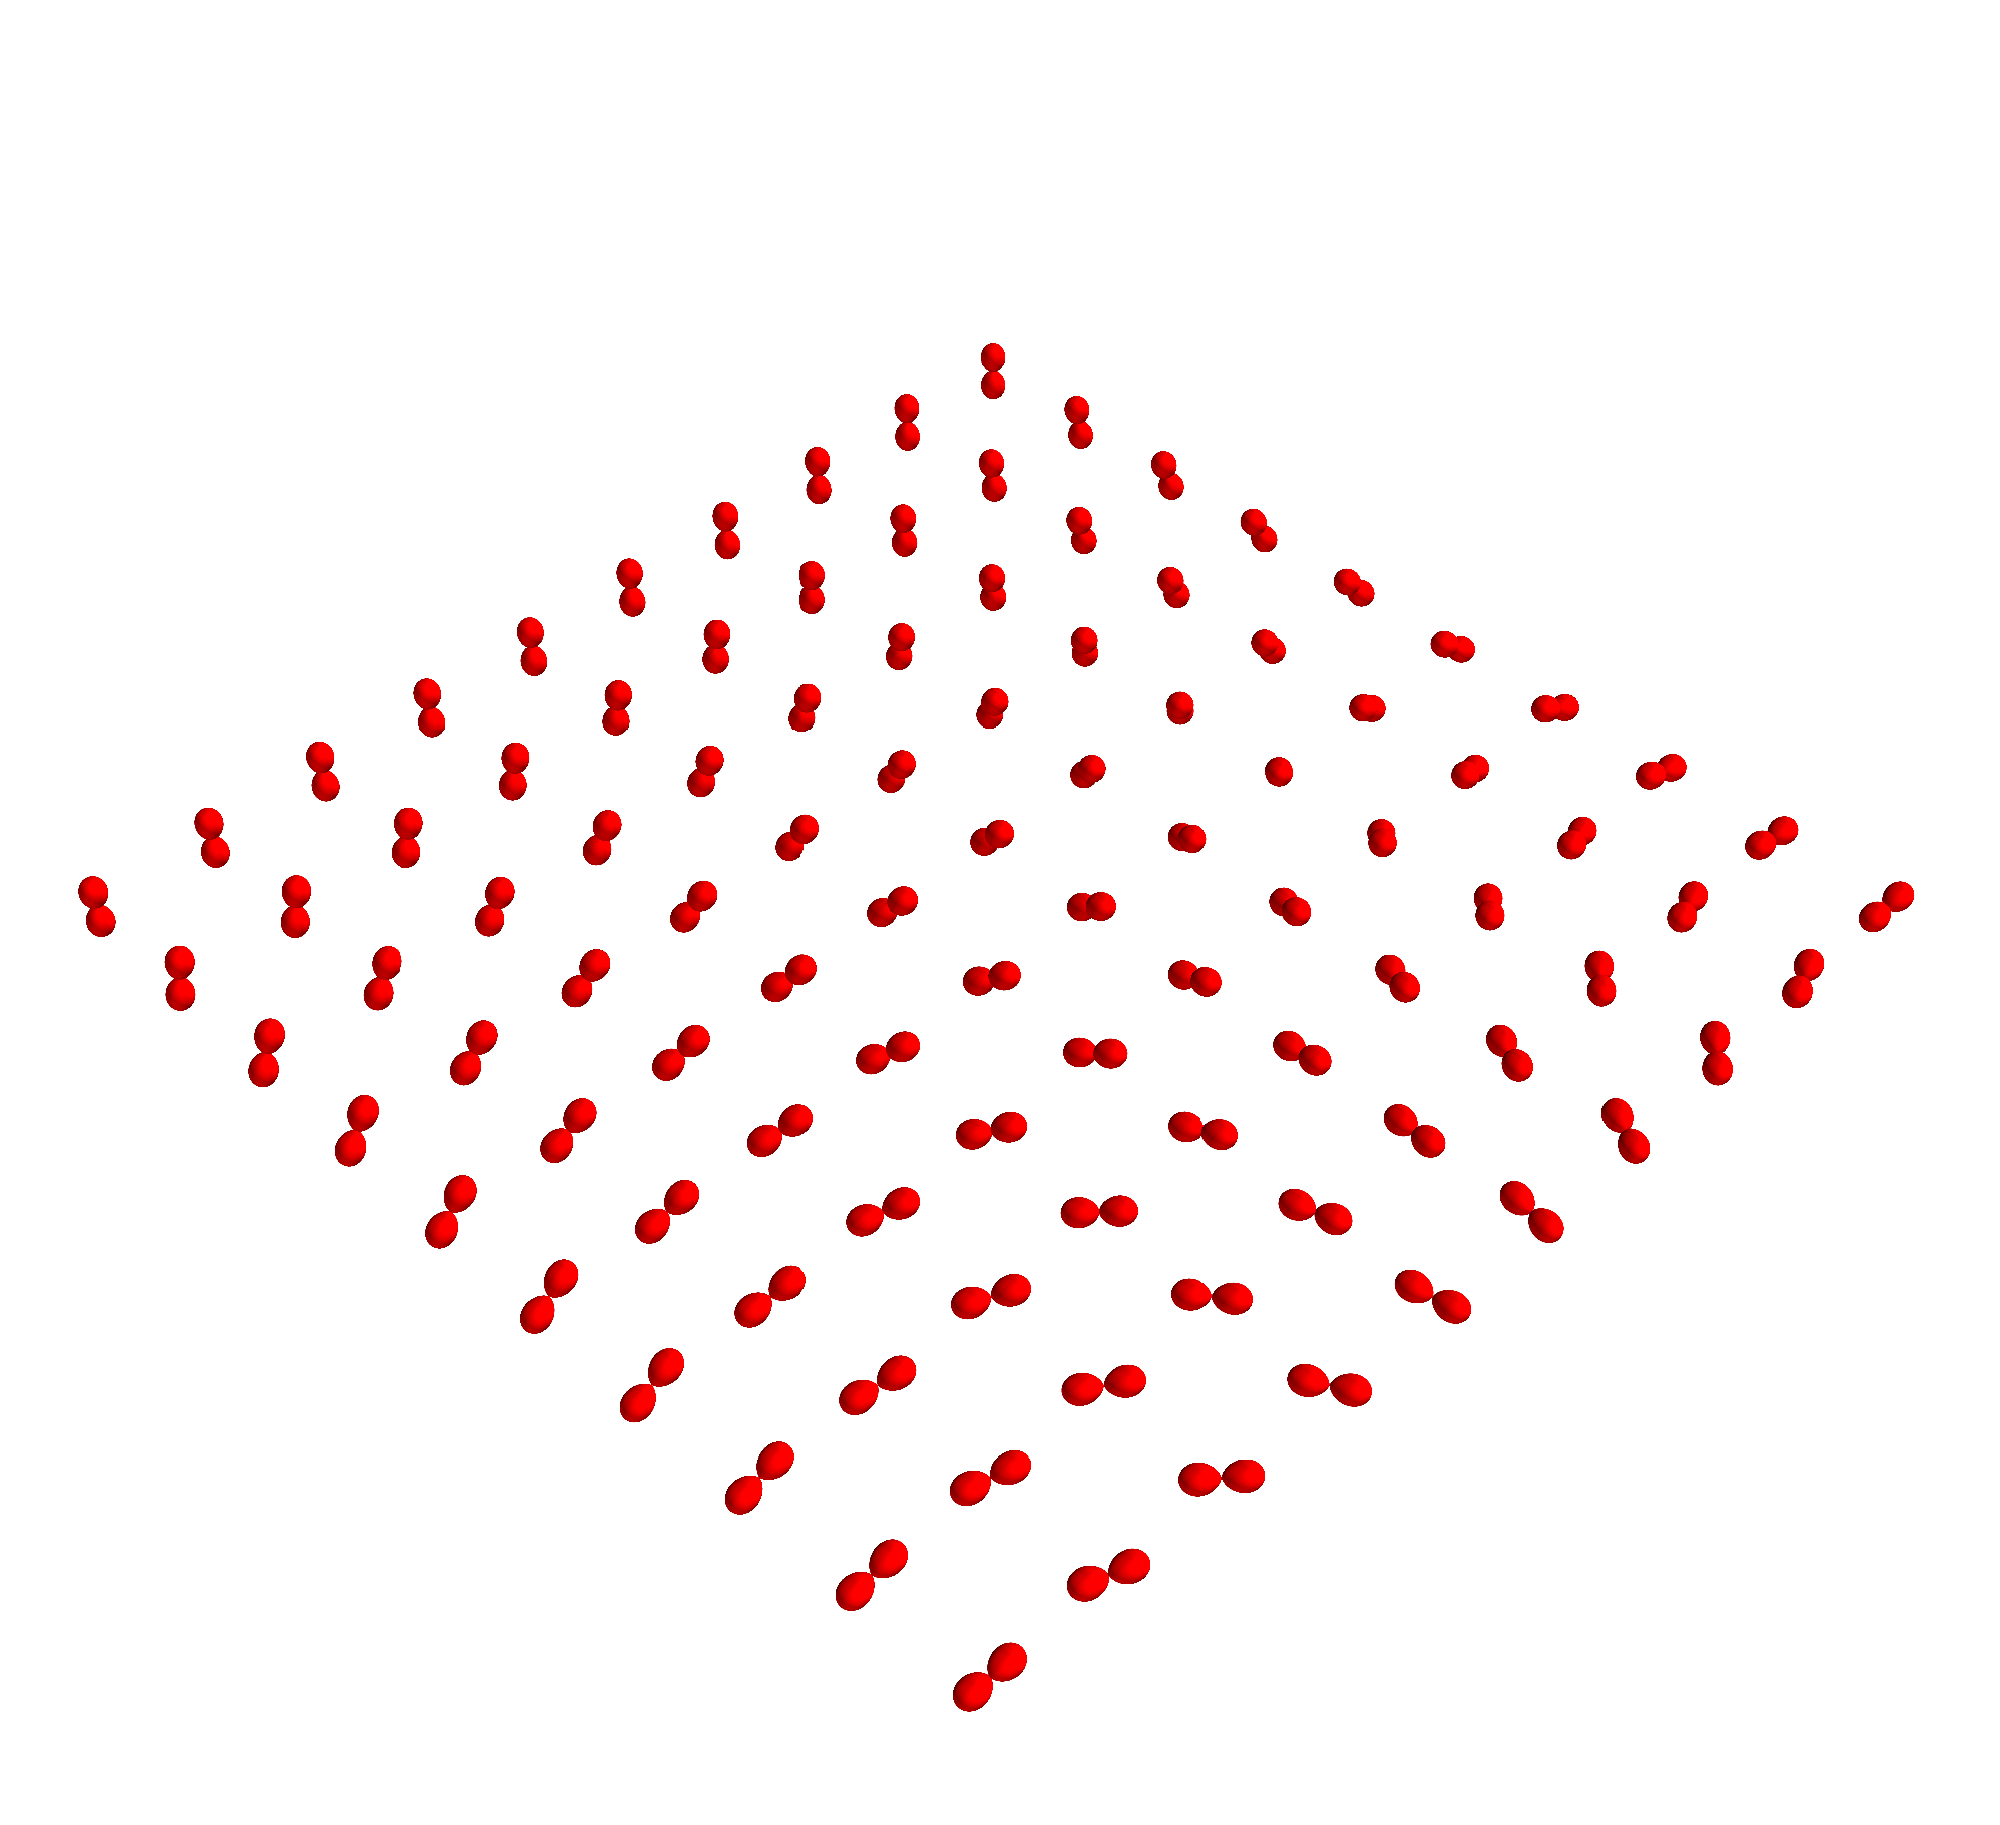
\includegraphics[width=0.7\textwidth, interpolate=true]{figs/phantom}}%
  \onslide<2>\centerline{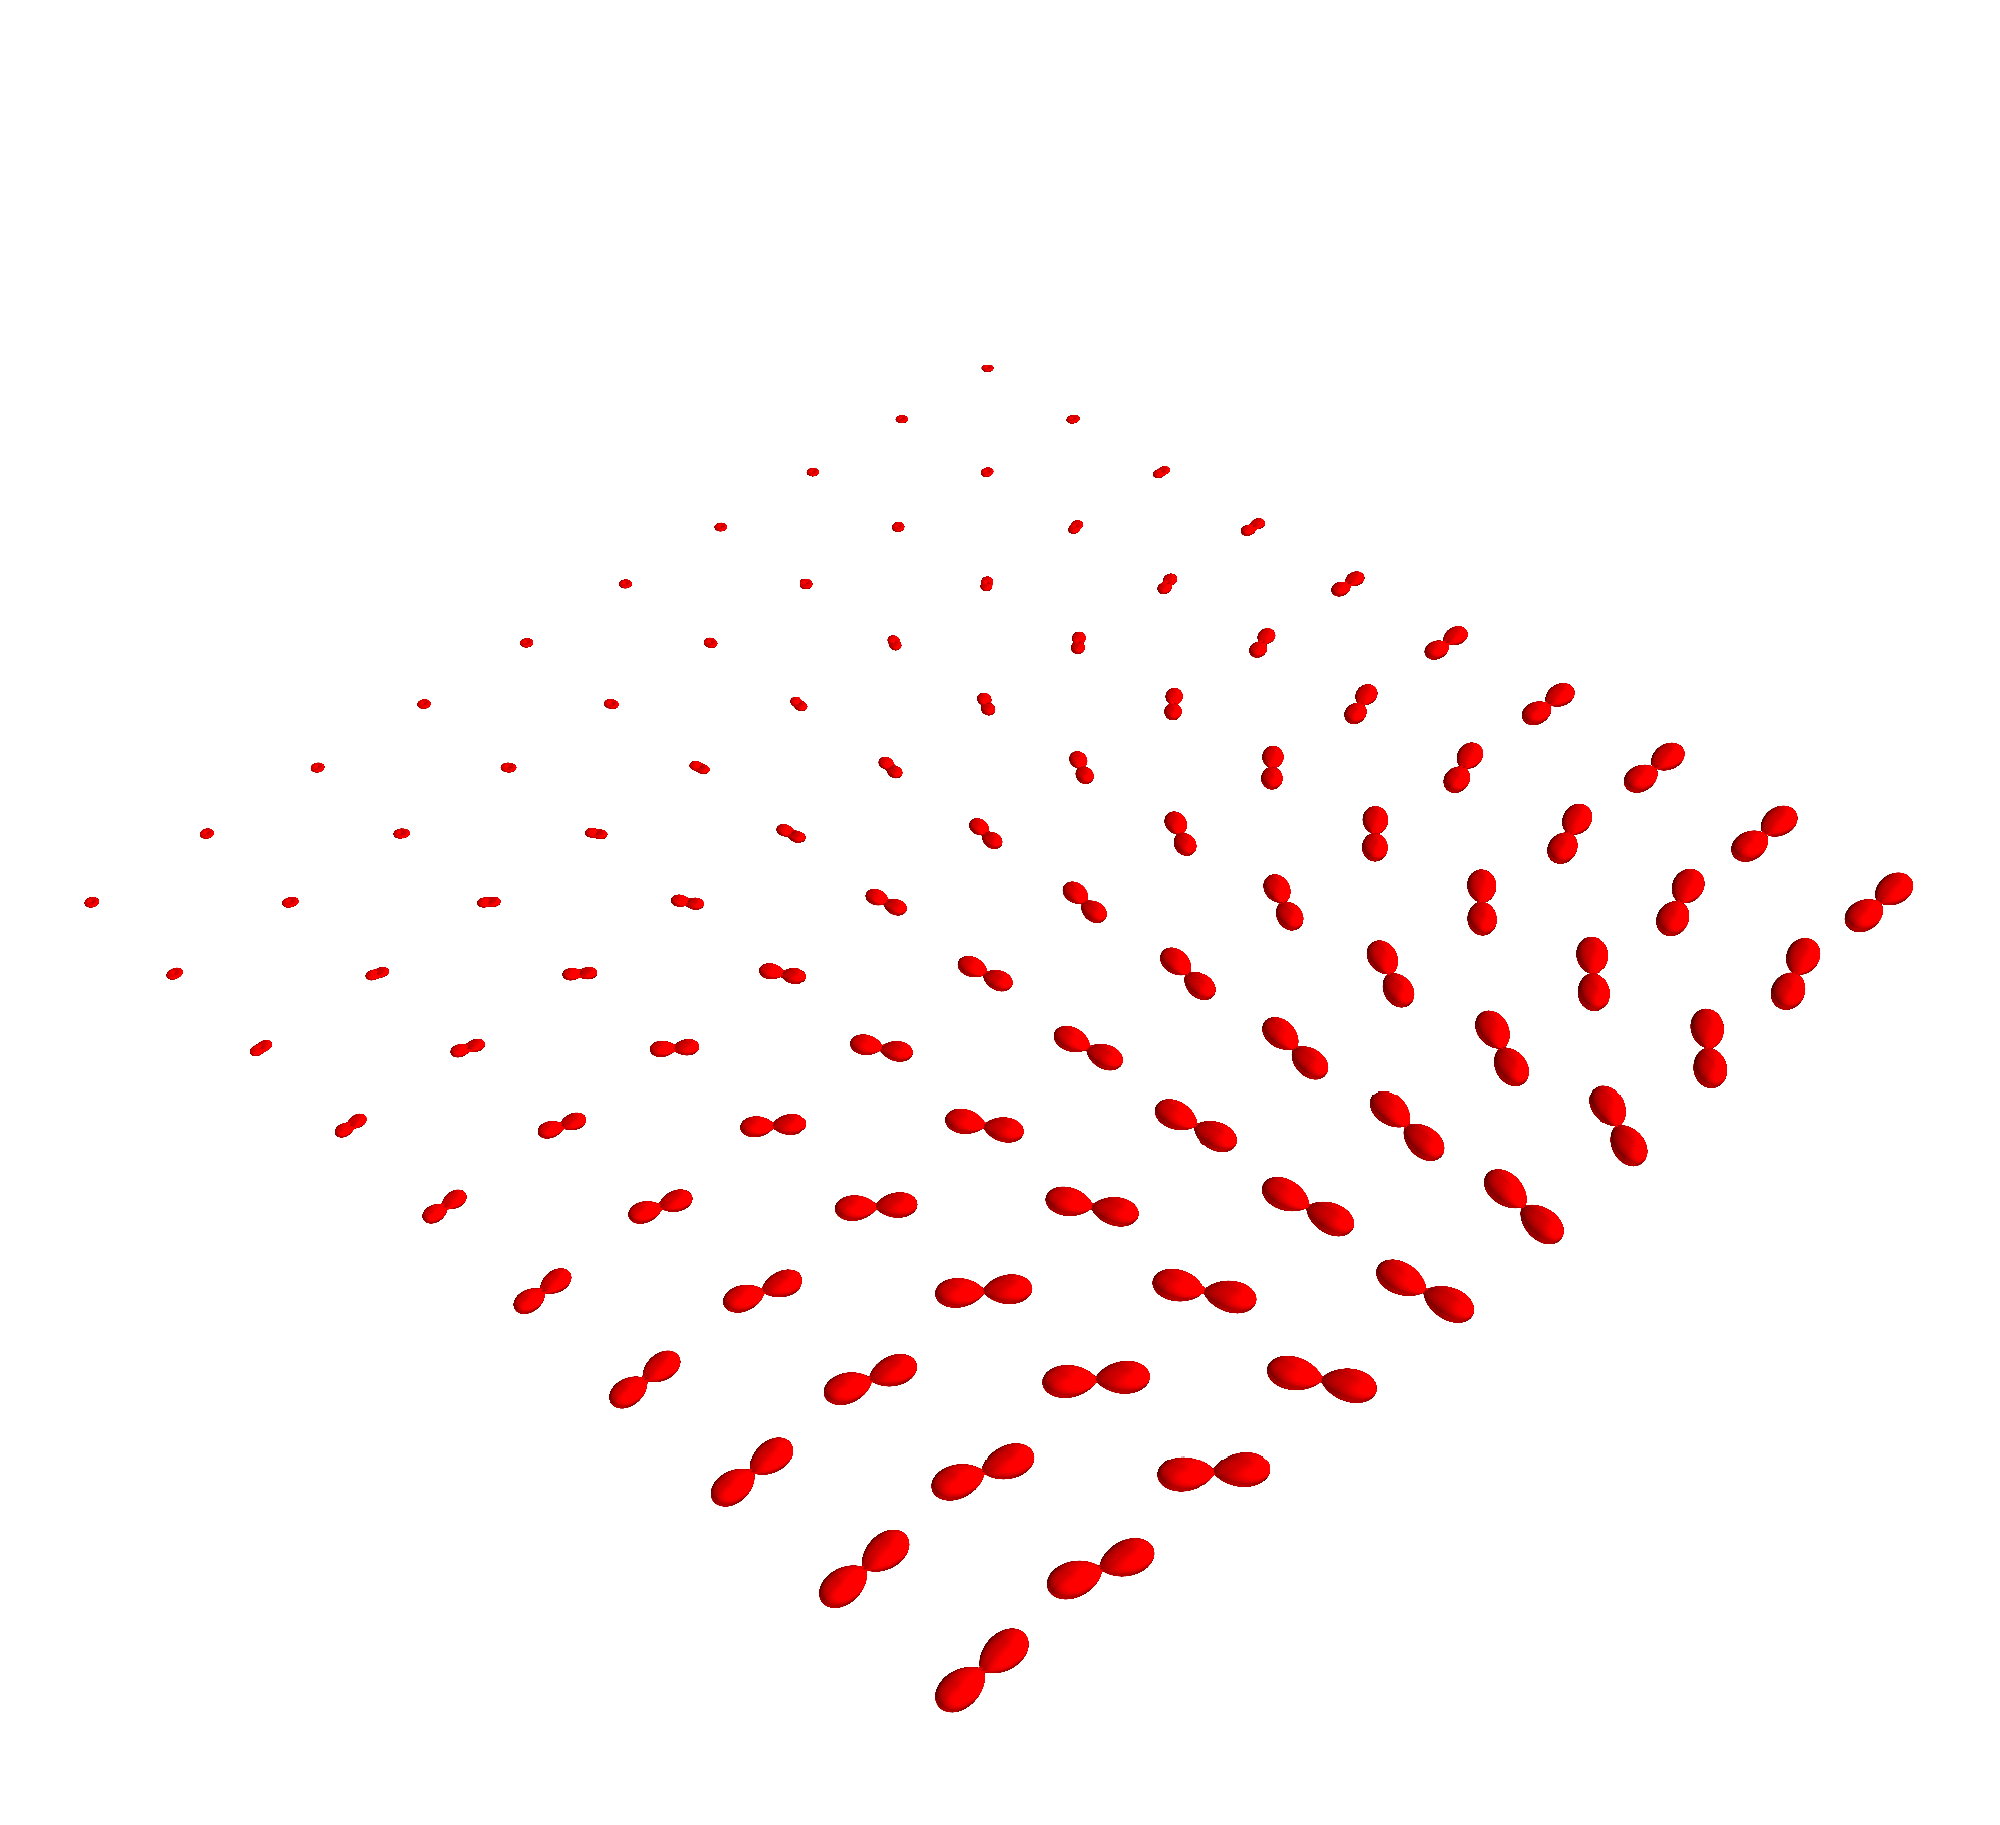
\includegraphics[width=0.7\textwidth, interpolate=true]{figs/phantom_epi_recon}}%
  \onslide<3>\centerline{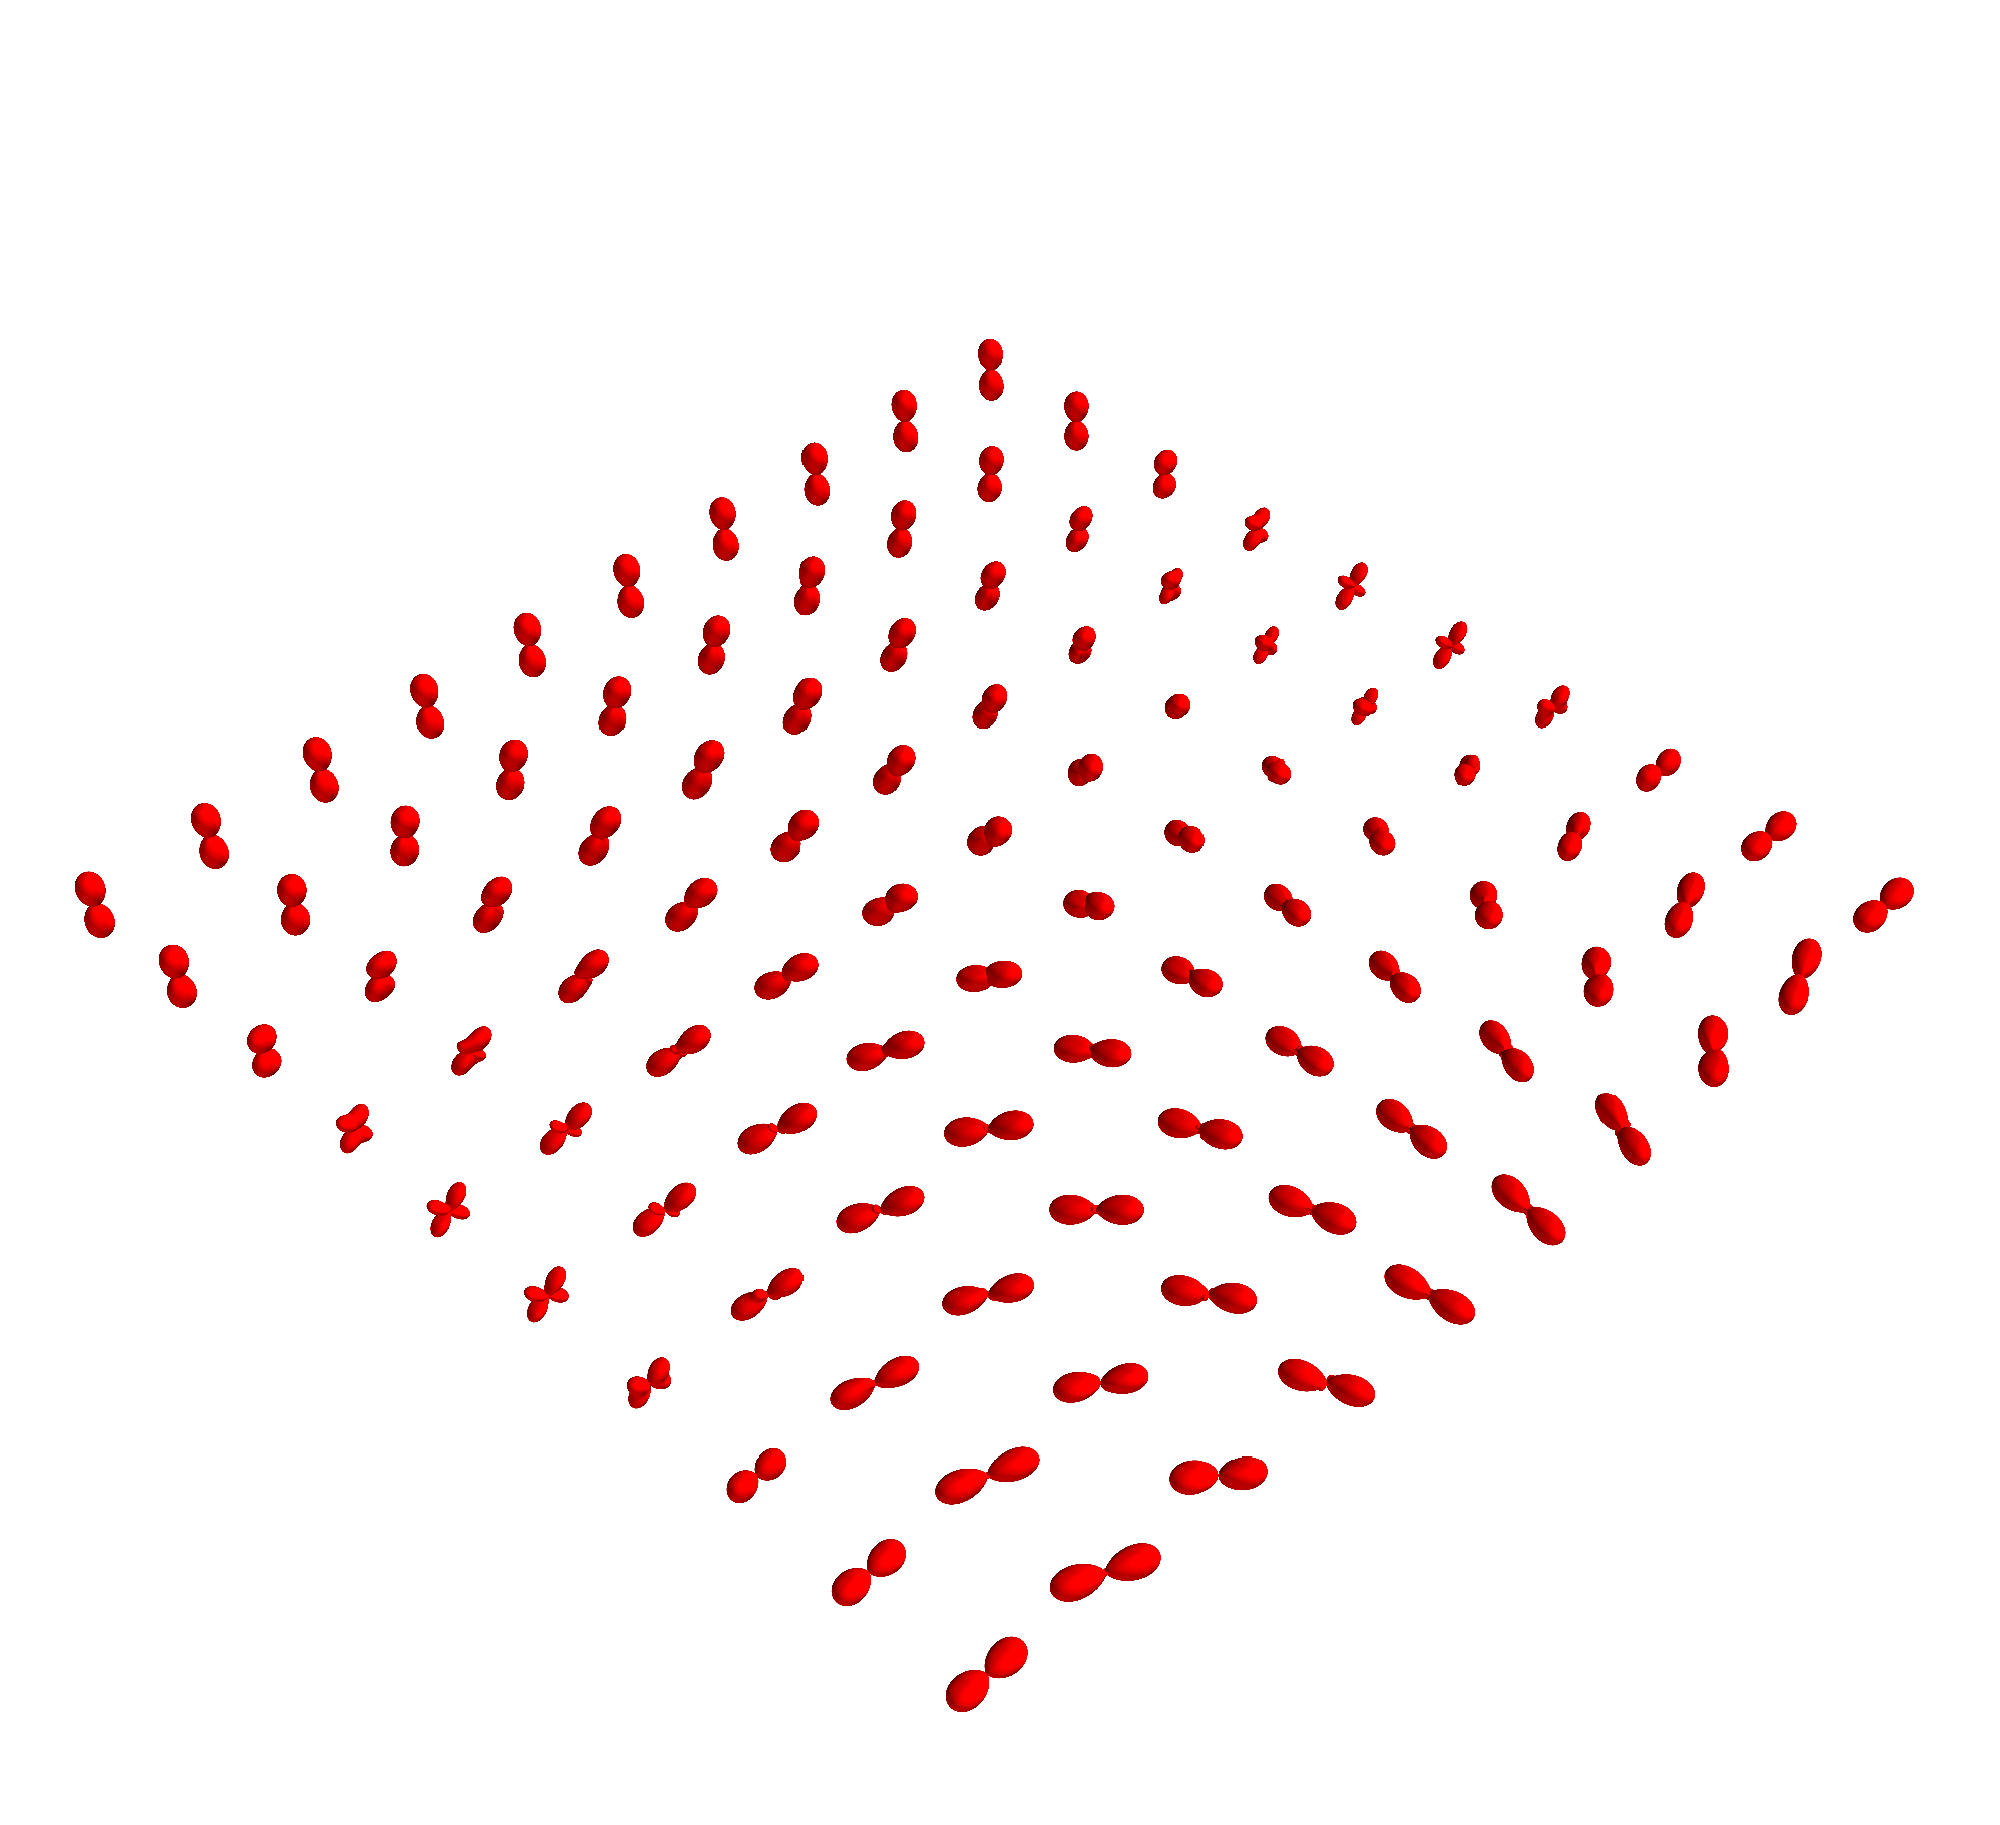
\includegraphics[width=0.7\textwidth, interpolate=true]{figs/phantom_dispim_recon}}%
\end{overprint}
\end{frame}


\begin{frame}{Reconstruction with priors}
    \begin{equation*}
    \begin{aligned}
      \mathbf{f^*} =\ \  
    & \underset{\mathbf{f}}{\text{argmin}}
    & & ||\mathbf{g} - \mathbf{\Psi}\mathbf{B}^+\mathbf{f}||_2^2 \\
    & \text{subject to}
    & & \mathbf{f} \in \text{prior set}
    \end{aligned}
  \end{equation*}
\end{frame}

% \begin{frame}{Single-view epi-illumination microscope NA = 0.8}
%   \begin{align*}
%   \mathbf{g} &= \mathbf{\Psi}\textbf{F}
%   \end{align*}
% \begin{center}
%   \includegraphics[width=1.0\textwidth, interpolate=true]{figs/epi/matrix}
% \end{center}
% \end{frame}

% \begin{frame}{Inverting A Rectangular Matrix}
%   \fontsize{10pt}{7.2}\selectfont
%   \begin{align*}
%     \under{N\times 1}{\mathbf{g}} &= \under{N\times M}{\mathbf{\Psi}}\under{M\times 1}{\mathbf{F}}
%     \intertext{Decompose $\mathbf{\Psi}$ into three matrices}
%                                     \under{N\times 1}{\mathbf{g}} &= \under{N\times N}{\mathbf{U}}\under{N\times M}{\mathbf{\Sigma}}\under{M\times M}{\mathbf{V}^T}\under{M\times 1}{\mathbf{F}}\\
%     \intertext{where $\mathbf{U}$ and $\mathbf{V}$ are orthogonal matrices---that is $\mathbf{U}^T = \mathbf{U}^{-1}$ or equivalently $\mathbf{U}^T\mathbf{U} = \mathbf{I}$---and $\mathbf{\Sigma}$ is a diagonal matrix. Solving for $\mathbf{F}$ gives}
%     \under{M\times 1}{\mathbf{F}} &= \under{M\times M}{\mathbf{V}}\under{M\times N}{\mathbf{\Sigma}^{-1}}\under{N\times N}{\mathbf{U}^T}\under{N\times 1}{\mathbf{g}}.\\
%     \intertext{But wait! $\mathbf{\Sigma}^{-1}$ doesn't exist. Instead, replace every element of $\mathbf{\Sigma}$ with its inverse (except the zeros), takes its transpose, and call it $\mathbf{\Sigma}^+$}
%     \under{M\times 1}{\mathbf{F}} &= \under{M\times M}{\mathbf{V}}\under{M\times N}{\mathbf{\Sigma}^{+}}\under{N\times N}{\mathbf{U}^T}\under{N\times 1}{\mathbf{g}}.\\
%     \intertext{This gives us the closest we can get to an inverse---the pseudo-inverse}
%     \under{M\times 1}{\mathbf{F}} &= \under{M\times N}{\mathbf{\Psi}^{+}}\under{N\times 1}{\mathbf{g}.}
%   \end{align*}
% \end{frame}

% \begin{frame}{Vocabulary}
%   \begin{align*}
%     \mathbf{\Psi}^{+}&\rightarrow \text{\textbf{pseudo-inverse} of}\ \mathbf{\Psi}\\
%     \mathbf{\Psi} = \mathbf{U\Sigma V}^T&\rightarrow \text{\textbf{singular-value decomposition} of}\ \mathbf{\Psi}\\
%     \text{Diagonal elements of}\ \mathbf{\Sigma}&\rightarrow \text{\textbf{singular values} of}\ \mathbf{\Psi}\\
%     \text{Columns of}\ \mathbf{V}&\rightarrow \text{\textbf{right singular vectors} of}\ \mathbf{\Psi}\\
%     \text{Columns of}\ \mathbf{U}&\rightarrow \text{\textbf{left singular vectors} of}\ \mathbf{\Psi}\\        
%   \end{align*}
% \end{frame}

% \begin{frame}{Single-view epi-illumination microscope NA = 0.8}
% \begin{center}
%   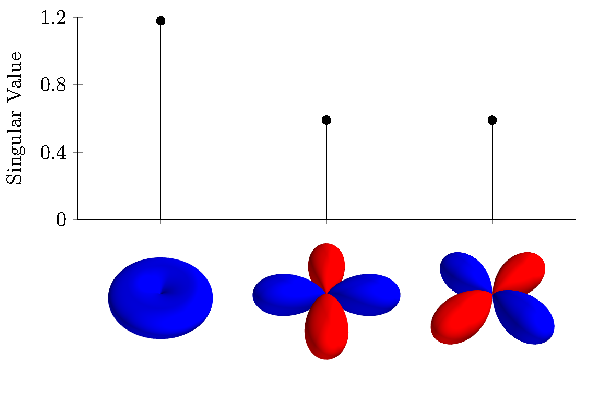
\includegraphics[width=0.8\textwidth, interpolate=true]{figs/svs_epi}
% \end{center}
% \end{frame}

% \begin{frame}{Symmetric diSPIM NA = 0.8}
% \begin{center}
%   \includegraphics[width=1.0\textwidth, interpolate=true]{figs/dispim/matrix}
% \end{center}
% \end{frame}

% \begin{frame}{Symmetric diSPIM, NA = 0.8}
% \begin{center}
%   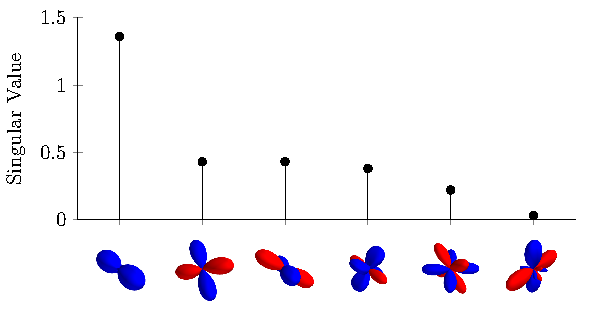
\includegraphics[width=0.8\textwidth, interpolate=true]{figs/svs_dispim}
% \end{center}
% \end{frame}

% \begin{frame}{Asymmetric diSPIM, NA = 1.1/0.7}
% \begin{center}
%   \includegraphics[width=1.0\textwidth, interpolate=true]{figs/dispim_asymmetric/matrix}
% \end{center}
% \end{frame}

% \begin{frame}{Asymmetric diSPIM NA = 1.1/0.7}
% \begin{center}
%   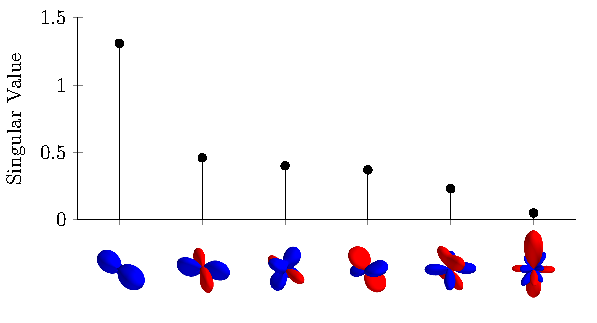
\includegraphics[width=0.8\textwidth, interpolate=true]{figs/svs_dispim_asym}
% \end{center}
% \end{frame}

% \begin{frame}{Test phantom - single fluorophores approximated by 7 degrees of spherical harmonics}
% \begin{center}
%   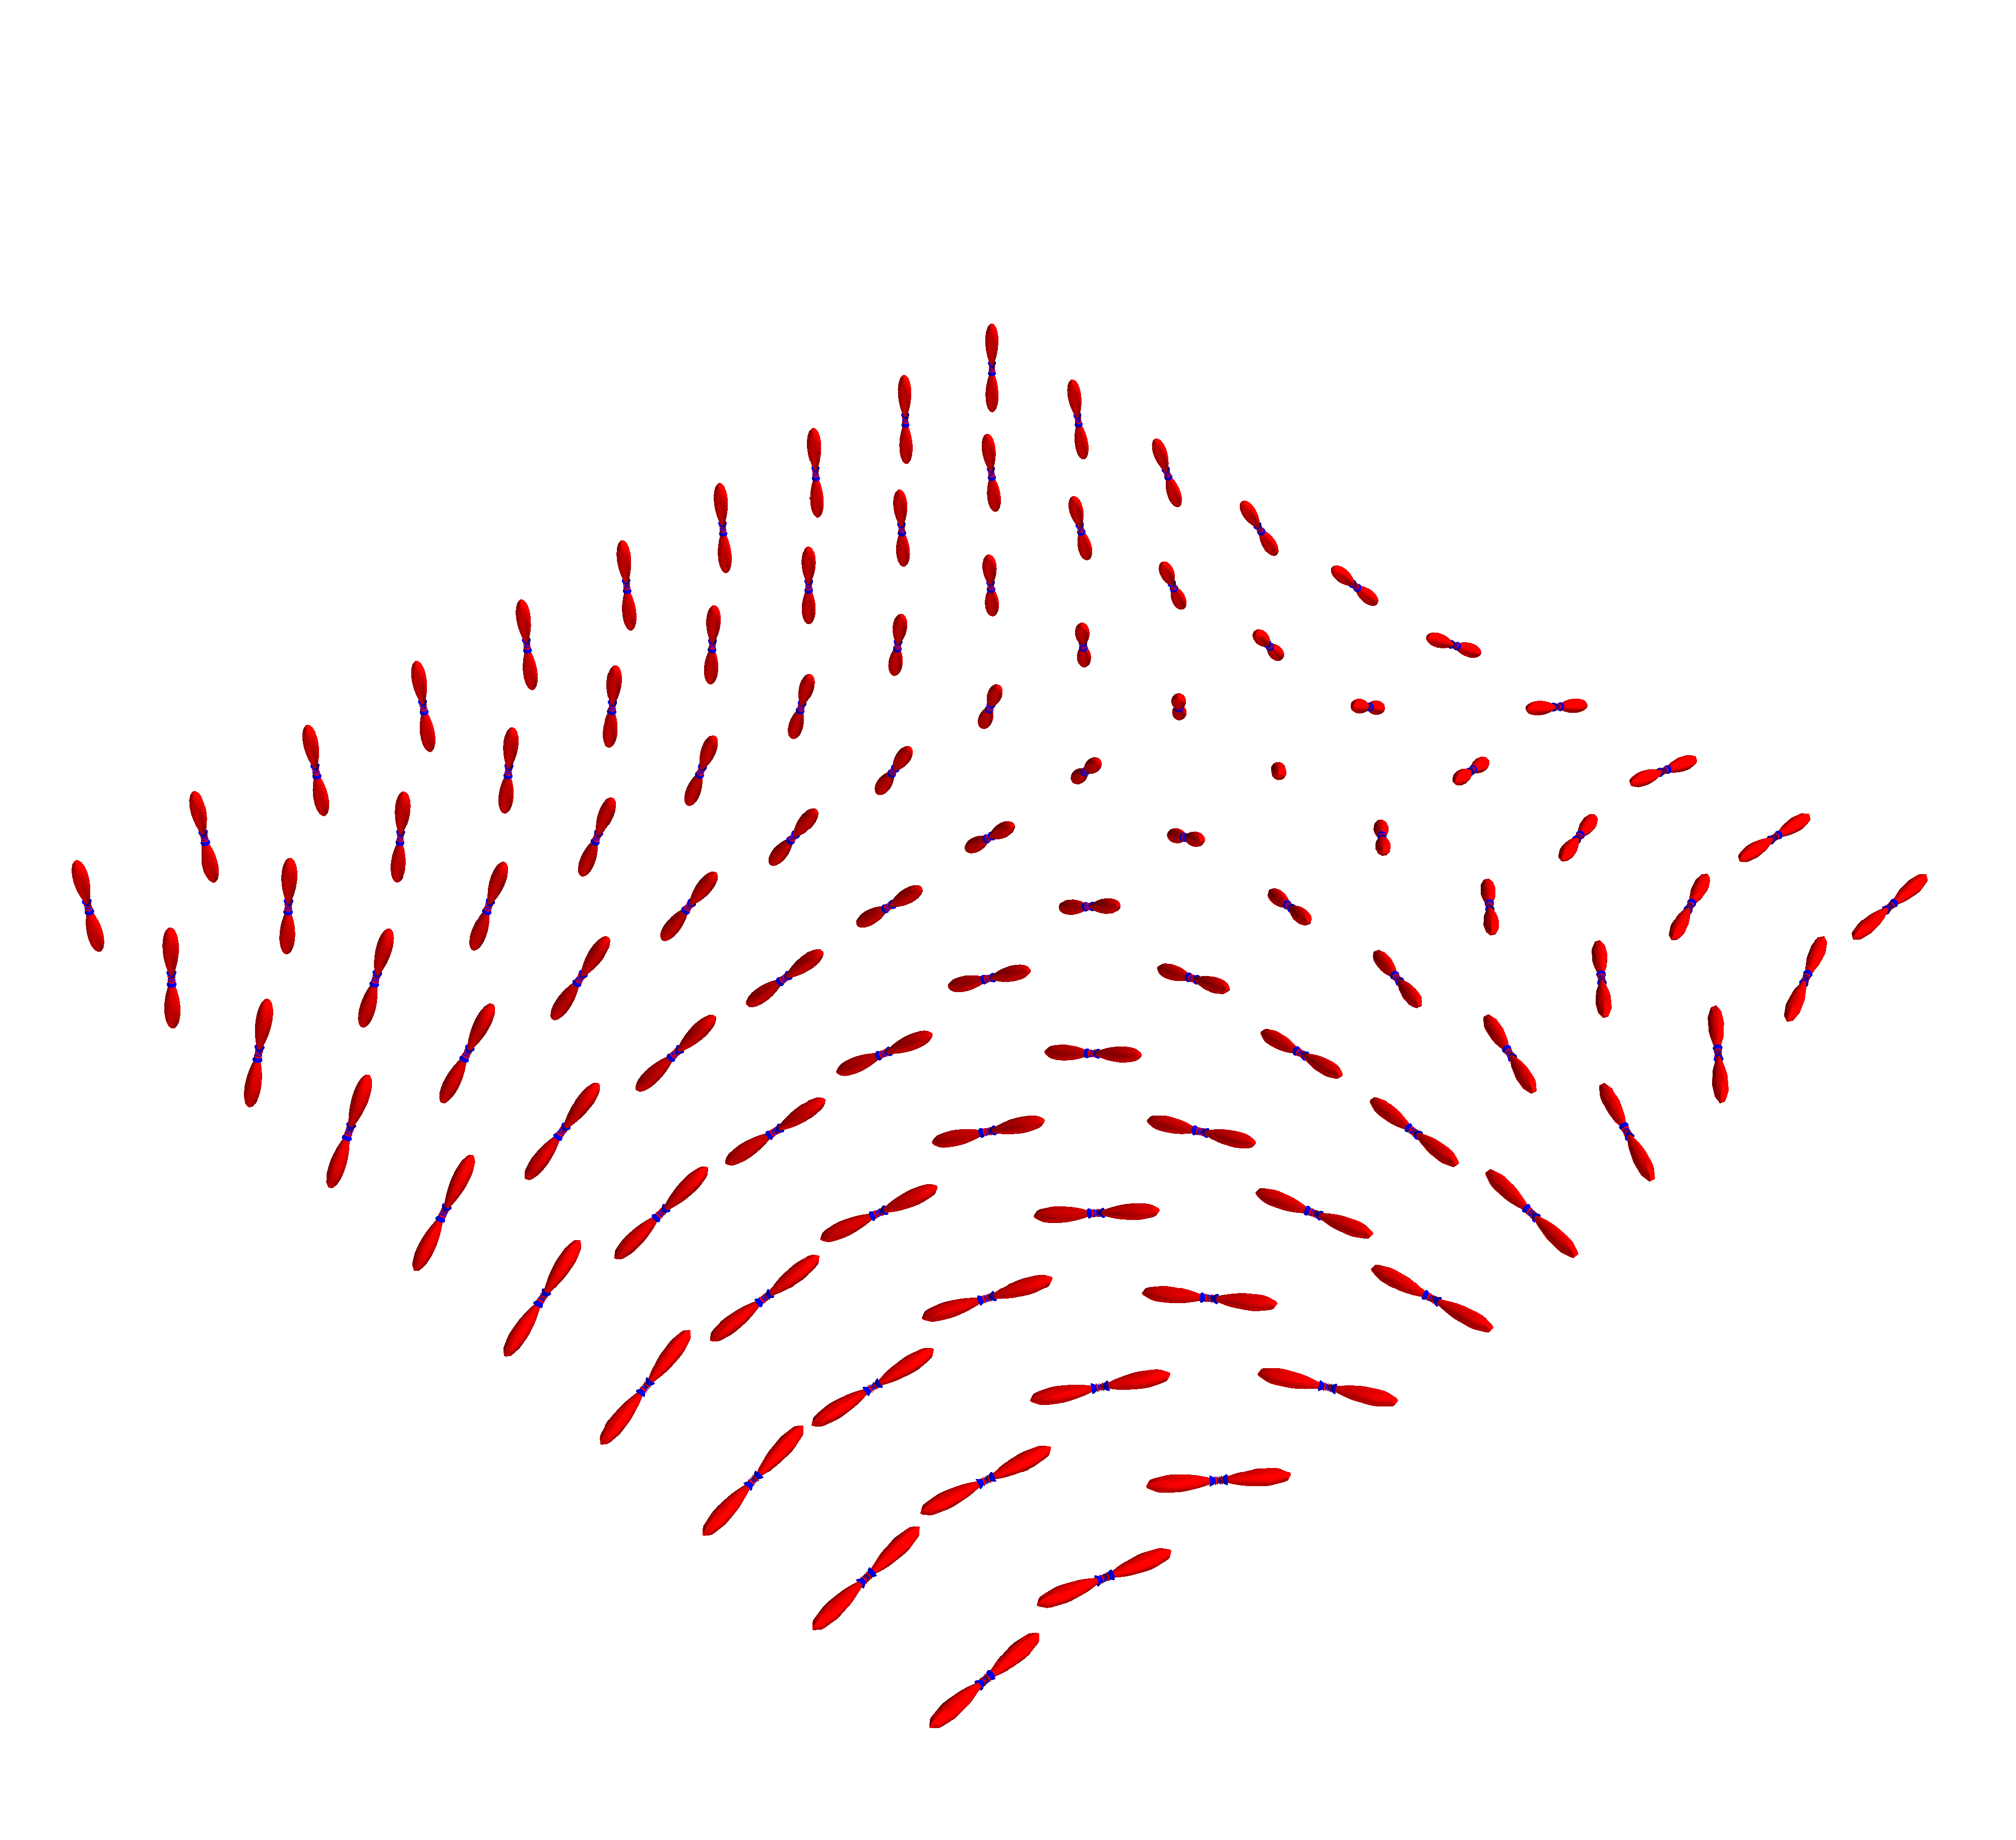
\includegraphics[width=0.8\textwidth, interpolate=true, trim={0 0 0 12cm}]{figs/tp_test.png}
% \end{center}
% \end{frame}

% \begin{frame}{Measured by the asymmetric diSPIM then reconstructed. No priors! Not even positivity ;)}
% \begin{center}
%   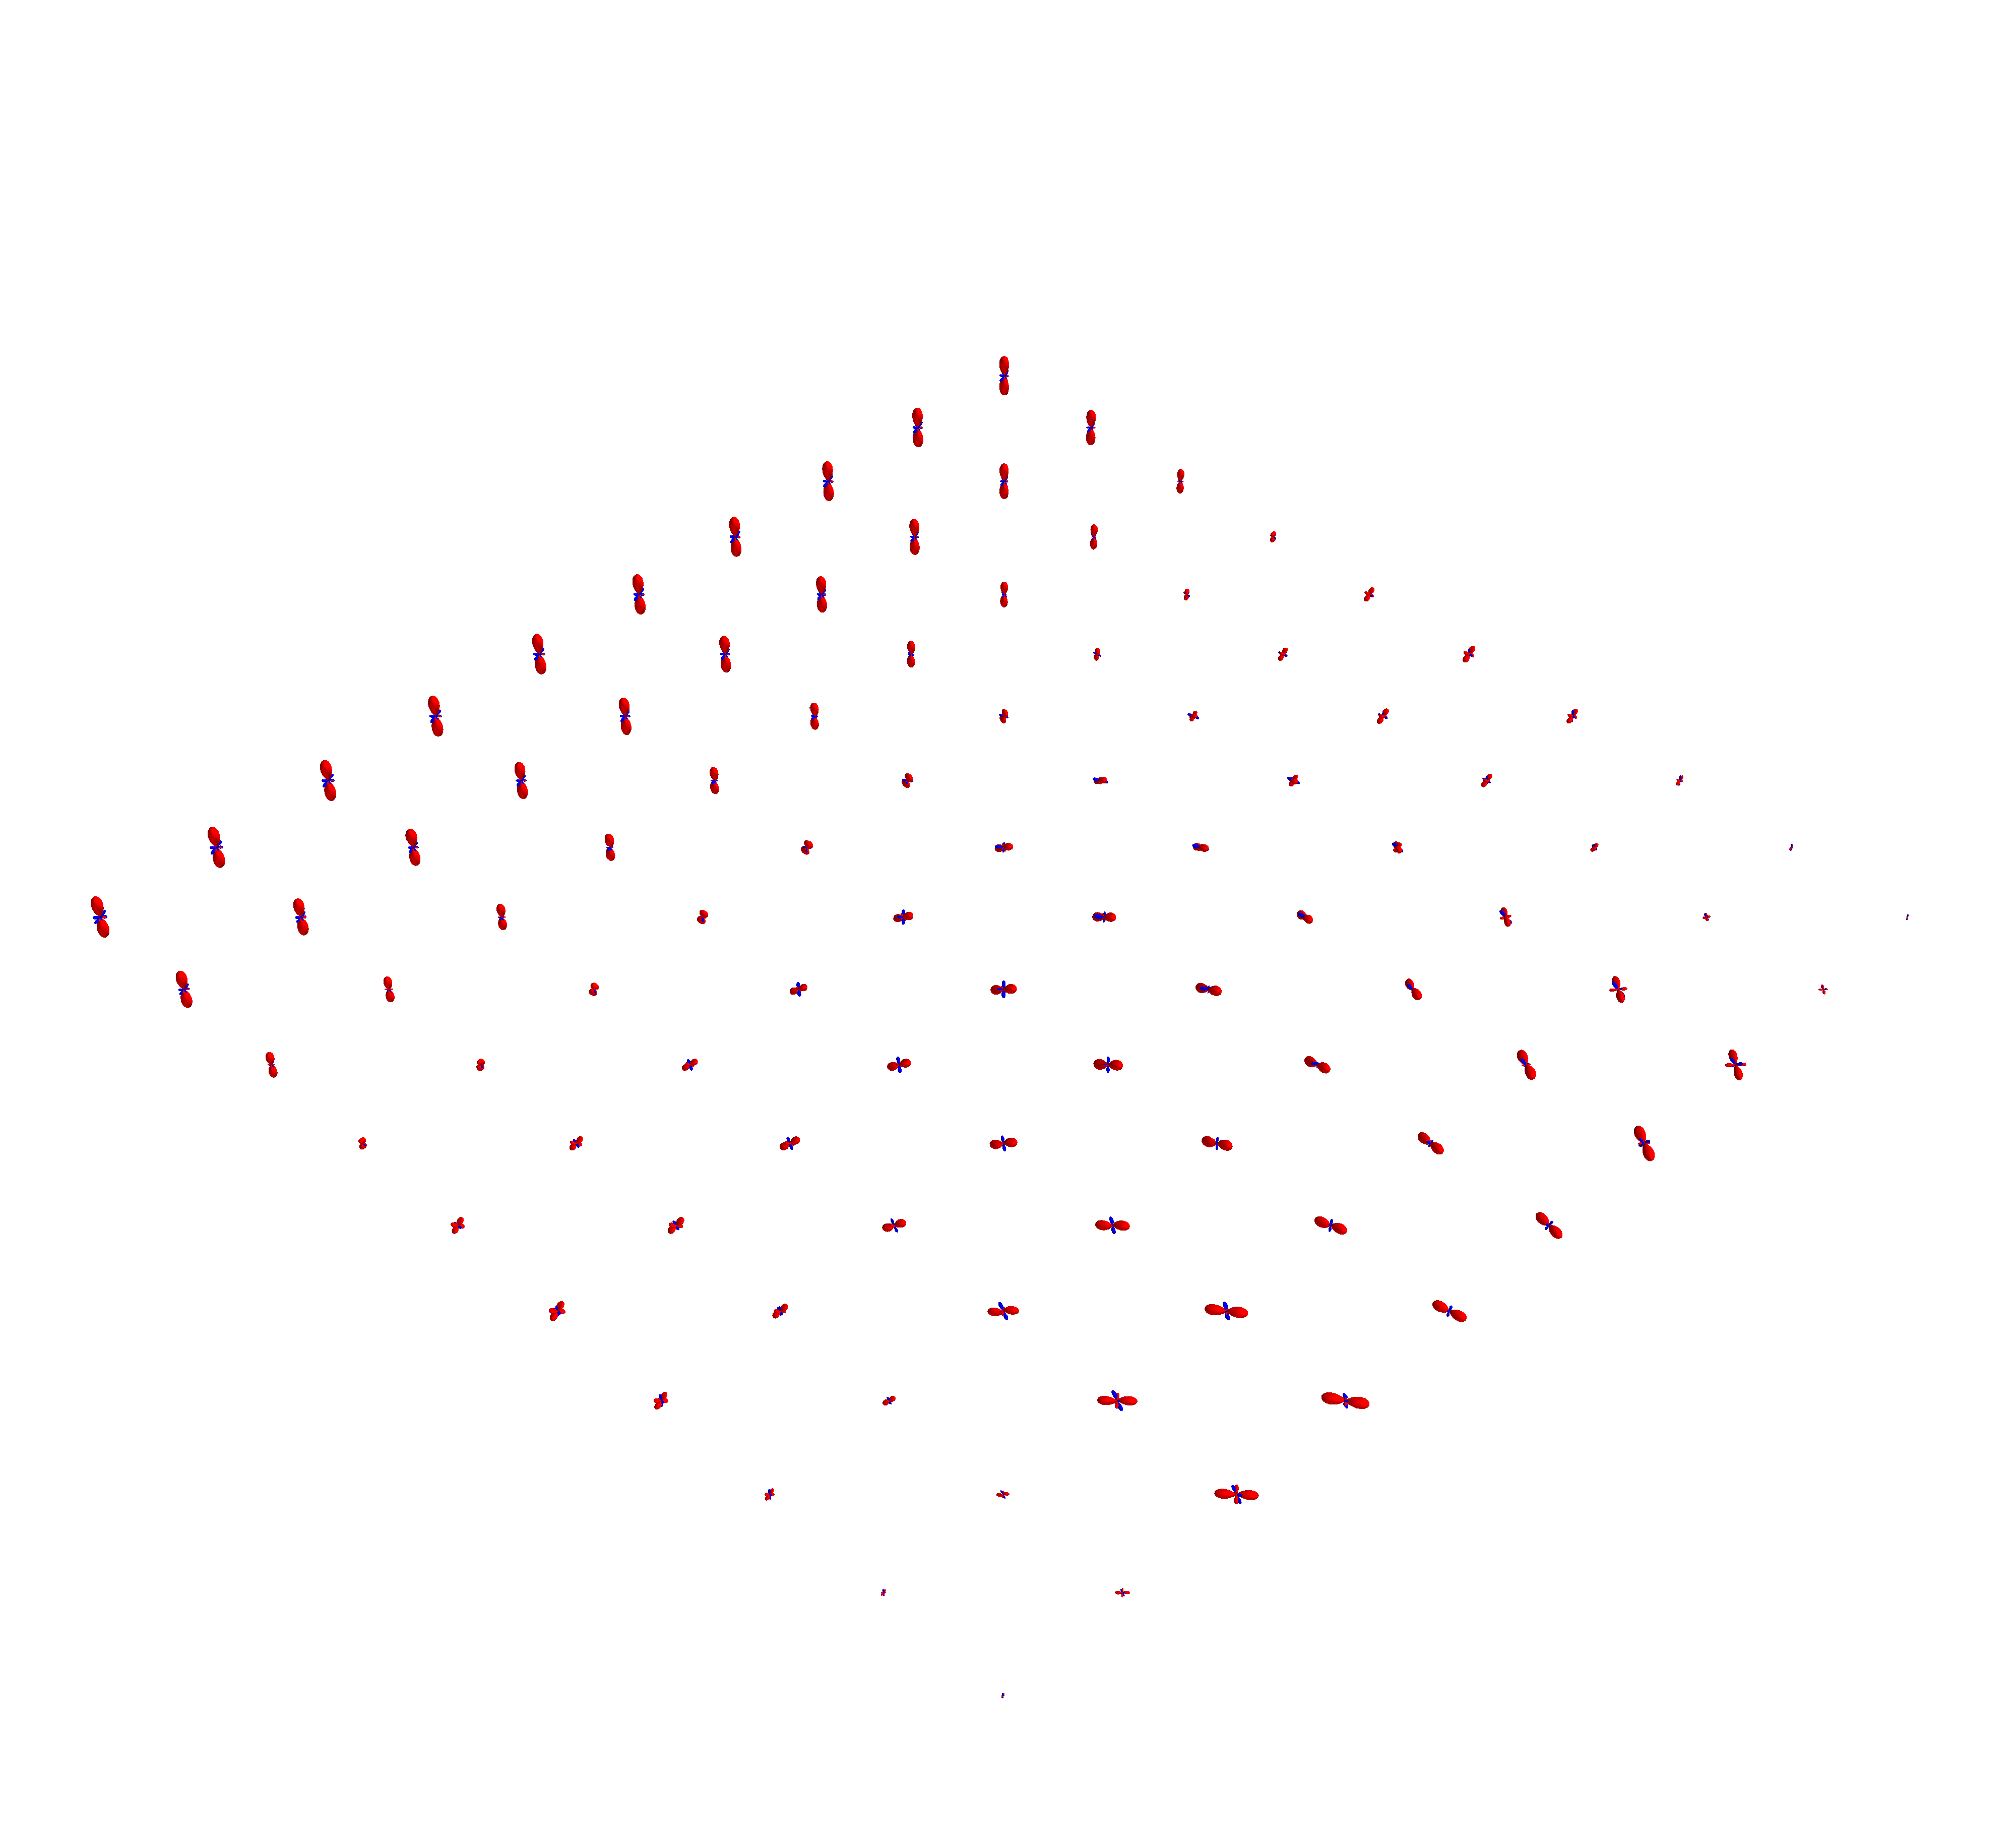
\includegraphics[width=0.8\textwidth, interpolate=true, trim={0 0 0 12cm}]{figs/recon_test.png}
% \end{center}
% \end{frame}

% \begin{frame}{Up Next}
%   \begin{itemize}
%   \item Incorporating priors---positivity, single fluorophore, rotational symmetry
%   \item Math OSA 2-page abstract on Jan 18---I'll include the work in these
%     slides. I'll possibly include priors depending on how quickly that goes.
%   \end{itemize}
% \end{frame}

% \begin{frame}[label=sec-12]{Giant Unilamallar Vesicles (GUV)\\ FOV $\approx$ 150 $\times$ 150 $\mu$\text{m}}
% \begin{center}
%   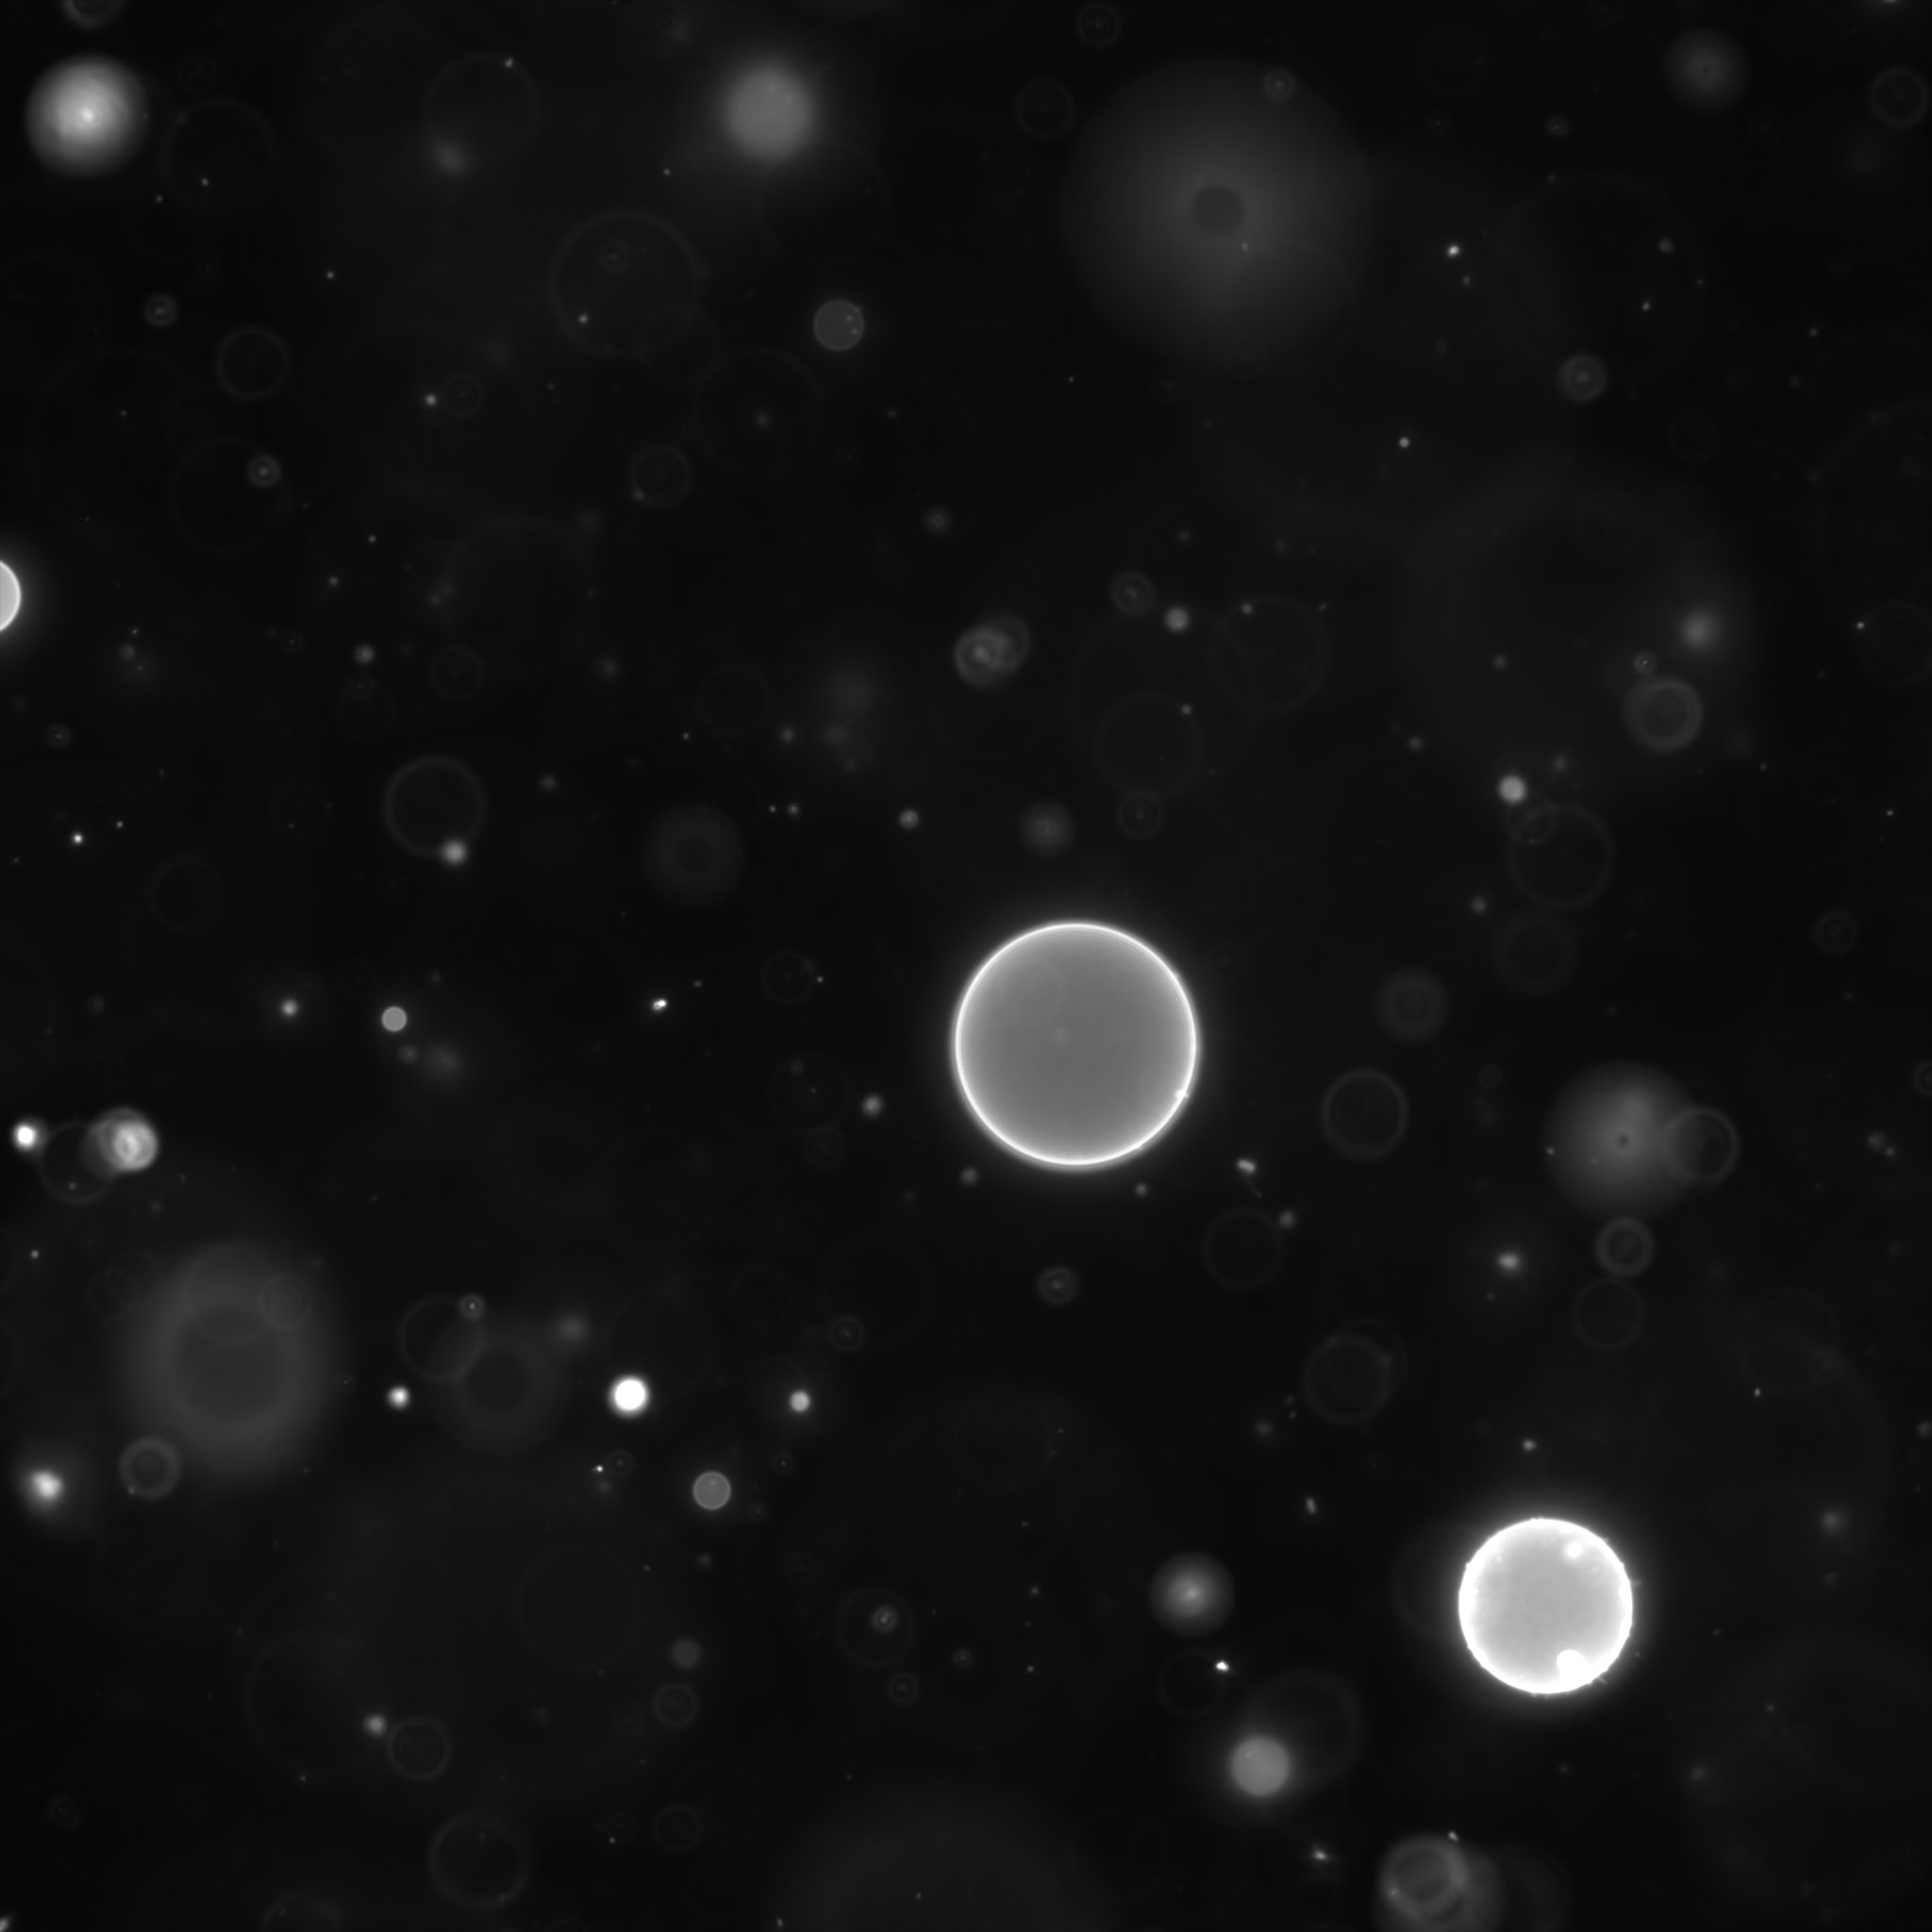
\includegraphics[width=0.6\textwidth, interpolate=true]{figs/guv.jpg}
% \end{center}
% \end{frame}
% \begin{frame}[label=sec-13]{GUV Protocol}
% \begin{center}
%   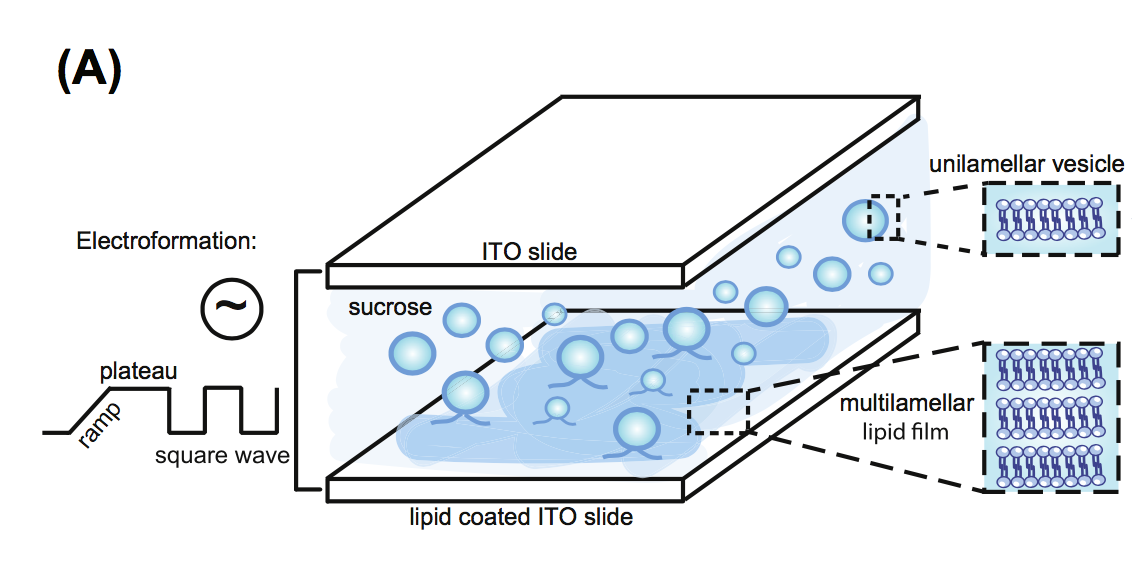
\includegraphics[width=0.9\textwidth, interpolate=true]{figs/schmid2015}
%   \raisebox{-10pt}{\makebox[0pt][r]{\footnotesize Schmid, 2015}}
% \end{center}
% \end{frame}

% \begin{frame}[label=sec-14]{GUV Chamber}
% \begin{center}
%   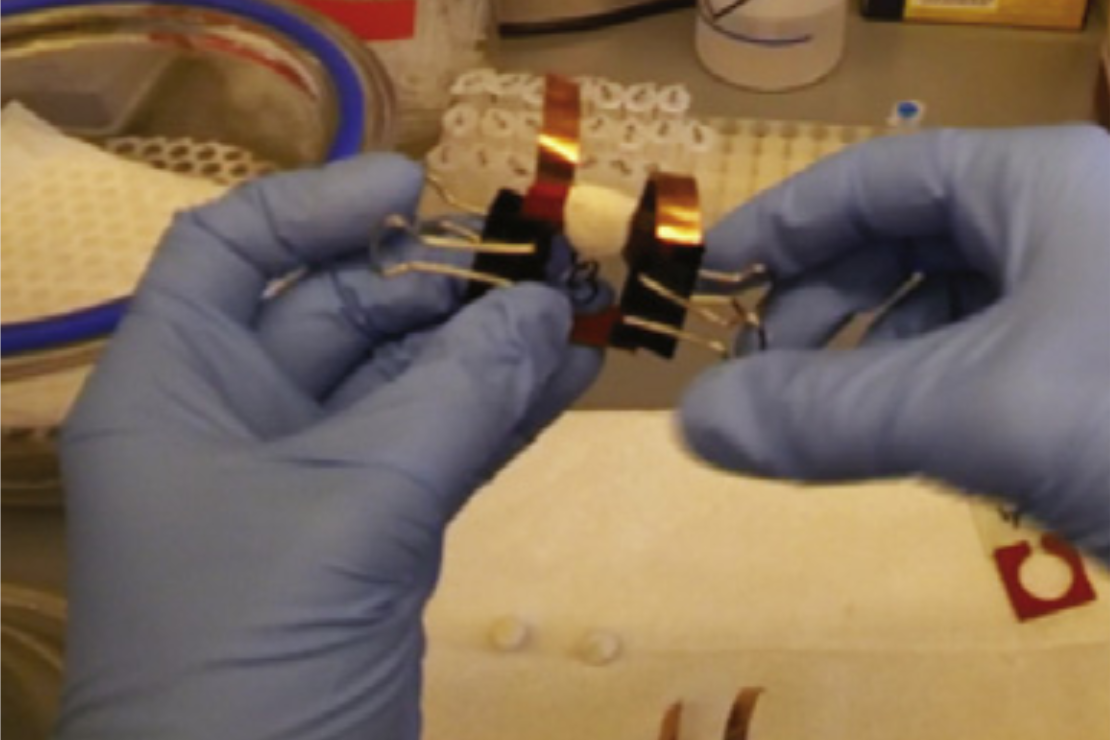
\includegraphics[width=0.7\textwidth, interpolate=true]{figs/chamber}
%   \raisebox{-10pt}{\makebox[0pt][r]{\footnotesize Schmid, 2015}}
% \end{center}
% \end{frame}
\end{document}